% Options for packages loaded elsewhere
\PassOptionsToPackage{unicode}{hyperref}
\PassOptionsToPackage{hyphens}{url}
%
\documentclass[
]{article}
\usepackage{amsmath,amssymb}
\usepackage{lmodern}
\usepackage{iftex}
\ifPDFTeX
  \usepackage[T1]{fontenc}
  \usepackage[utf8]{inputenc}
  \usepackage{textcomp} % provide euro and other symbols
\else % if luatex or xetex
  \usepackage{unicode-math}
  \defaultfontfeatures{Scale=MatchLowercase}
  \defaultfontfeatures[\rmfamily]{Ligatures=TeX,Scale=1}
\fi
% Use upquote if available, for straight quotes in verbatim environments
\IfFileExists{upquote.sty}{\usepackage{upquote}}{}
\IfFileExists{microtype.sty}{% use microtype if available
  \usepackage[]{microtype}
  \UseMicrotypeSet[protrusion]{basicmath} % disable protrusion for tt fonts
}{}
\makeatletter
\@ifundefined{KOMAClassName}{% if non-KOMA class
  \IfFileExists{parskip.sty}{%
    \usepackage{parskip}
  }{% else
    \setlength{\parindent}{0pt}
    \setlength{\parskip}{6pt plus 2pt minus 1pt}}
}{% if KOMA class
  \KOMAoptions{parskip=half}}
\makeatother
\usepackage{xcolor}
\usepackage[margin=1in]{geometry}
\usepackage{color}
\usepackage{fancyvrb}
\newcommand{\VerbBar}{|}
\newcommand{\VERB}{\Verb[commandchars=\\\{\}]}
\DefineVerbatimEnvironment{Highlighting}{Verbatim}{commandchars=\\\{\}}
% Add ',fontsize=\small' for more characters per line
\usepackage{framed}
\definecolor{shadecolor}{RGB}{248,248,248}
\newenvironment{Shaded}{\begin{snugshade}}{\end{snugshade}}
\newcommand{\AlertTok}[1]{\textcolor[rgb]{0.94,0.16,0.16}{#1}}
\newcommand{\AnnotationTok}[1]{\textcolor[rgb]{0.56,0.35,0.01}{\textbf{\textit{#1}}}}
\newcommand{\AttributeTok}[1]{\textcolor[rgb]{0.77,0.63,0.00}{#1}}
\newcommand{\BaseNTok}[1]{\textcolor[rgb]{0.00,0.00,0.81}{#1}}
\newcommand{\BuiltInTok}[1]{#1}
\newcommand{\CharTok}[1]{\textcolor[rgb]{0.31,0.60,0.02}{#1}}
\newcommand{\CommentTok}[1]{\textcolor[rgb]{0.56,0.35,0.01}{\textit{#1}}}
\newcommand{\CommentVarTok}[1]{\textcolor[rgb]{0.56,0.35,0.01}{\textbf{\textit{#1}}}}
\newcommand{\ConstantTok}[1]{\textcolor[rgb]{0.00,0.00,0.00}{#1}}
\newcommand{\ControlFlowTok}[1]{\textcolor[rgb]{0.13,0.29,0.53}{\textbf{#1}}}
\newcommand{\DataTypeTok}[1]{\textcolor[rgb]{0.13,0.29,0.53}{#1}}
\newcommand{\DecValTok}[1]{\textcolor[rgb]{0.00,0.00,0.81}{#1}}
\newcommand{\DocumentationTok}[1]{\textcolor[rgb]{0.56,0.35,0.01}{\textbf{\textit{#1}}}}
\newcommand{\ErrorTok}[1]{\textcolor[rgb]{0.64,0.00,0.00}{\textbf{#1}}}
\newcommand{\ExtensionTok}[1]{#1}
\newcommand{\FloatTok}[1]{\textcolor[rgb]{0.00,0.00,0.81}{#1}}
\newcommand{\FunctionTok}[1]{\textcolor[rgb]{0.00,0.00,0.00}{#1}}
\newcommand{\ImportTok}[1]{#1}
\newcommand{\InformationTok}[1]{\textcolor[rgb]{0.56,0.35,0.01}{\textbf{\textit{#1}}}}
\newcommand{\KeywordTok}[1]{\textcolor[rgb]{0.13,0.29,0.53}{\textbf{#1}}}
\newcommand{\NormalTok}[1]{#1}
\newcommand{\OperatorTok}[1]{\textcolor[rgb]{0.81,0.36,0.00}{\textbf{#1}}}
\newcommand{\OtherTok}[1]{\textcolor[rgb]{0.56,0.35,0.01}{#1}}
\newcommand{\PreprocessorTok}[1]{\textcolor[rgb]{0.56,0.35,0.01}{\textit{#1}}}
\newcommand{\RegionMarkerTok}[1]{#1}
\newcommand{\SpecialCharTok}[1]{\textcolor[rgb]{0.00,0.00,0.00}{#1}}
\newcommand{\SpecialStringTok}[1]{\textcolor[rgb]{0.31,0.60,0.02}{#1}}
\newcommand{\StringTok}[1]{\textcolor[rgb]{0.31,0.60,0.02}{#1}}
\newcommand{\VariableTok}[1]{\textcolor[rgb]{0.00,0.00,0.00}{#1}}
\newcommand{\VerbatimStringTok}[1]{\textcolor[rgb]{0.31,0.60,0.02}{#1}}
\newcommand{\WarningTok}[1]{\textcolor[rgb]{0.56,0.35,0.01}{\textbf{\textit{#1}}}}
\usepackage{graphicx}
\makeatletter
\def\maxwidth{\ifdim\Gin@nat@width>\linewidth\linewidth\else\Gin@nat@width\fi}
\def\maxheight{\ifdim\Gin@nat@height>\textheight\textheight\else\Gin@nat@height\fi}
\makeatother
% Scale images if necessary, so that they will not overflow the page
% margins by default, and it is still possible to overwrite the defaults
% using explicit options in \includegraphics[width, height, ...]{}
\setkeys{Gin}{width=\maxwidth,height=\maxheight,keepaspectratio}
% Set default figure placement to htbp
\makeatletter
\def\fps@figure{htbp}
\makeatother
\setlength{\emergencystretch}{3em} % prevent overfull lines
\providecommand{\tightlist}{%
  \setlength{\itemsep}{0pt}\setlength{\parskip}{0pt}}
\setcounter{secnumdepth}{-\maxdimen} % remove section numbering
\usepackage[english]{babel}
\DeclareUnicodeCharacter{308}{oe}
\ifLuaTeX
  \usepackage{selnolig}  % disable illegal ligatures
\fi
\IfFileExists{bookmark.sty}{\usepackage{bookmark}}{\usepackage{hyperref}}
\IfFileExists{xurl.sty}{\usepackage{xurl}}{} % add URL line breaks if available
\urlstyle{same} % disable monospaced font for URLs
\hypersetup{
  pdftitle={Projectreport Machine Learning 2},
  pdfauthor={Maluna Menke, Ari (Sara) Wahl, Pavlo Kravets},
  hidelinks,
  pdfcreator={LaTeX via pandoc}}

\title{Projectreport Machine Learning 2}
\author{Maluna Menke, Ari (Sara) Wahl, Pavlo Kravets}
\date{2023-12-31}

\begin{document}
\maketitle

{
\setcounter{tocdepth}{6}
\tableofcontents
}
\pagenumbering{gobble}
\newpage
\pagenumbering{arabic} 
\centering
\raggedright
\newpage

\begin{center}\rule{0.5\linewidth}{0.5pt}\end{center}

\hypertarget{introduction}{%
\subsubsection{1. Introduction}\label{introduction}}

Our general idea was to work with LGBT-related data. This was not as
easy as expected, since it seems there are not a lot of datasets openly
available that have that kind of information. Finally, we found a US
survey by the CDC, that regularly monitors the country's youth in a lot
of dimensions, but among other questions also asks for sexual
experiences and identification.

\hypertarget{the-dataset}{%
\subsubsection{2. The Dataset}\label{the-dataset}}

\hfill\break
``The
\emph{\href{https://www.cdc.gov/healthyyouth/data/yrbs/data.htm}{Youth
Risk Behavior Survey (YRBS)}} measures health-related behaviors and
experiences that can lead to death and disability among youth and
adults.{[}\ldots{]} Some of the health-related behaviors and experiences
monitored are: - Student demographics: sex, sexual identity, race and
ethnicity, and grade - Youth health behaviors and conditions: sexual,
injury and violence, bullying, diet and physical activity, obesity, and
mental health, including suicide - Substance use behaviors: electronic
vapor product and tobacco product use, alcohol use, and other drug use -
Student experiences: parental monitoring, school connectedness, unstable
housing, and exposure to community violence
\protect\hyperlink{1}{{[}1{]}}. It is a national survey conducted by the
CDC (Center for Disease Control and Prevention) and includes high school
students from both private and public schools within the U.S. Data is
collected from 1991 through 2021, we are only using the most recent data
from 2021. If you want to learn more about the data there is an
accompanying Data User Guide.\protect\hyperlink{2}{{[}2{]}}.

\hypertarget{preprocessing-of-the-dataset}{%
\paragraph{2.1 Preprocessing of the
dataset}\label{preprocessing-of-the-dataset}}

\hfill\break

To preprocess the dataset, we first ran a summary of our dataset. The
number of NAs seems to depend very much on the question. The variable
``orig\_rec'' only contained NAs and has therefore been removed, as well
as the variable ``site'' which only contained ``XX'' entries. Variables
q4 and q5 are already aggregated in ``raceeth'' and have also been
deleted. The variable ``record'' seems to be an ID for the observations.
This has to be considered later.

\hypertarget{missing-data}{%
\paragraph{2.2 Missing Data}\label{missing-data}}

\hfill\break
We will first exclude all the observations with NAs in all the
target-related variables q25 to q29. Since we want to build our target
variable on these questions, the target variable cannot all be empty.
The amount of data available should be enough to just exclude these
observations. After removing the observations that have NAs in all the
variables, that are used to create our target variable, we still have
around 13.7\% NAs in the dataset.\\
What if we had just excluded every NA in the dataset? We will try and
see if this is a viable option, since this woul not just be quick and
easy, but we would also just have ``real'' answers. The exclusion of NAs
leads to a severe reduction in the number of observations. The original
data consisted of 17232 observations, after reducing the target-related
NAs only, we have 11753 observations left. If we omit all NAs, the
reduced dataframe still has 4334 observations.\\

In this case need to assess the loss of information foremost about our
target variable. The important question is if there is a pattern to the
missingness in our data, not just, but especially about our target
variable.

\hypertarget{omitting-nas-vs-data-imputation}{%
\paragraph{2.2.2 Omitting NAs vs Data
Imputation}\label{omitting-nas-vs-data-imputation}}

\hfill\break
If we can omit the NAs or if it may be necessary to impute the missing
data points, depends on the type of missingness. If data is missing
completely at random (MCAR), we can omit the NAs, if it is just missing
at random (MAR) we would rather impute the data. If the data is missing
not at random (MNAR), it would be a quite difficult problem because we
cannot easily impute the missing data then. To find out if we can just
omit the data, an MCAR test was applied.\\
We test the target-related variables q25 to q29 for potential pattern(s)
in the missing data. This results in a p-value of 0, which means we can
say for sure, that the data is not missing completely at random. Just
omitting all NAs could be problematic and lead to bias.\\

\begin{Shaded}
\begin{Highlighting}[]
\NormalTok{result }\OtherTok{\textless{}{-}} \FunctionTok{mcar\_test}\NormalTok{(RISK[, }\FunctionTok{c}\NormalTok{(}\StringTok{"q25"}\NormalTok{, }\StringTok{"q26"}\NormalTok{, }\StringTok{"q27"}\NormalTok{, }\StringTok{"q28"}\NormalTok{, }\StringTok{"q29"}\NormalTok{)])}
\FunctionTok{print}\NormalTok{(result)}
\end{Highlighting}
\end{Shaded}

\begin{verbatim}
## # A tibble: 1 x 4
##   statistic    df p.value missing.patterns
##       <dbl> <dbl>   <dbl>            <int>
## 1      452.    68       0               29
\end{verbatim}

Because of this, we will use a rule base approach to create the target
variable and impute the predictive variables afterwards. To ensure a
good imputation, we need to impute our NAs before reducing the dataset
to 2000 observations. To run the imputation properly we need to
factorize our nominal and ordinal variables first.

\hypertarget{target-variable}{%
\paragraph{2.3 Target Variable}\label{target-variable}}

\hfill\break
As a target variable, we decided to calculate a score from 5 questions
that reflect the suicide risk of the person (observation) in question.
This score is aggregated with a rule-based approach.

~ After creating the target variable we need to exclude the variables
q25 to q29, which were used for creating it, from our dataset.

\hypertarget{imputation}{%
\paragraph{2.4 Imputation}\label{imputation}}

\hypertarget{reducing-and-balancing-the-dataset-to-2000-observations}{%
\paragraph{2.5 Reducing and balancing the dataset to 2000
observations}\label{reducing-and-balancing-the-dataset-to-2000-observations}}

\hfill\break
We need to reduce our data to the maximum allowed size of 2000
observations. To ensure the best possible data quality, we want to
ensure that our dataset is balanced. Intuitively, we are considering if
it is best to still use as much of the non-imputed data for our smaller
dataset as possible, before filling it up with imputed data, since
non-imputed data is usually of better quality. On the other hand the
data seemingly shows patterns in the missingness so there are reasons to
just do a stratified sampling over the imputed data as well. To do a
proper statified sampling we need to identify the stratification
variables. Therefore we will calculate the correlations with the target
variable and see which variables are highly correlated to our target
variable. These will then as well as the target variable be used as
stratification variables.

\hypertarget{simple-synopsis-of-the-dataset}{%
\paragraph{2.6 Simple Synopsis of the
Dataset}\label{simple-synopsis-of-the-dataset}}

\hfill\break
number of observations: 2000 number of variables: 100

datatypes: factor: 96 - nominal variables: 29 - ordinal variables: 67
numeric variables: 4 - discrete variables: 96 (here all factor
variables) - continuous variables: 4 (here all numeric variables)

\hypertarget{additional-data-preparation}{%
\subsubsection{3. Additional Data
Preparation}\label{additional-data-preparation}}

question: would it introduce information leakage to reduce the features
before splitting the data?

\hypertarget{feature-reduction}{%
\paragraph{3.1 Feature Reduction}\label{feature-reduction}}

\hfill\break
Since our dataset has lots of variables, we decided to start by
excluding some variables depending on the estimated feature importance.

\hypertarget{correlations}{%
\paragraph{3.1.1 Correlations}\label{correlations}}

~ Unfortunately at this point we have to many variables to do a pairs
plot or correlation plot with a visually usable outcome. We will
therefore perform a correlation analysis only with respect to the target
variable and in numeric format instead of any visual plot.

\begin{verbatim}
## Rows: 1998 Columns: 86
## -- Column specification --------------------------------------------------------
## Delimiter: ","
## chr  (1): q7orig
## dbl (85): raceeth, q6orig, q1, q2, q3, q6, q7, q8, q9, q10, q11, q14, q16, q...
## 
## i Use `spec()` to retrieve the full column specification for this data.
## i Specify the column types or set `show_col_types = FALSE` to quiet this message.
\end{verbatim}

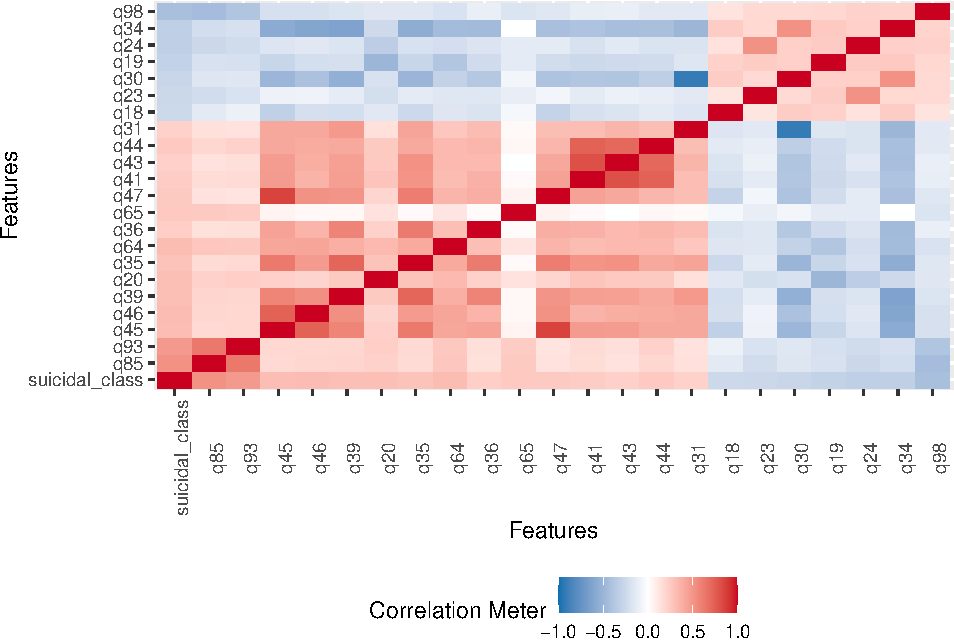
\includegraphics{report_pdf_files/figure-latex/corr plot-1.pdf}

\begin{Shaded}
\begin{Highlighting}[]
\FunctionTok{print}\NormalTok{(corr\_vars)}
\end{Highlighting}
\end{Shaded}

\begin{verbatim}
##  [1] "suicidal_class" "Prob"           "q85"            "q93"           
##  [5] "q45"            "q64"            "q39"            "q20"           
##  [9] "q65"            "q35"            "q36"            "q49"           
## [13] "q47"            "q46"            "q30"            "q86"           
## [17] "q23"            "q76"            "q34"            "q19"           
## [21] "q24"            "q98"            "Stratum"
\end{verbatim}

The 18 variables with high correlations (\textgreater0.25) with our
target variable are: q93\\
q85\\
q45\\
q35\\
q36\\
q39\\
q64\\
q46\\
q20\\
q30\\
q24\\
q19\\
q98\\
q34 q41 q43 q44 q47

\hypertarget{feature-selection-algorithm}{%
\paragraph{3.1.2 Feature Selection
Algorithm}\label{feature-selection-algorithm}}

Since the data still has a lot of variables, we need to use a feature
selection technique to reduce the features before using a machine
learning method. We chose to use model agnostic methods, because the
feature selection should be valid for all methods that are later
compared. In an earlier step the variables most correlated with the
target variable were already identified. Unfortunately this captures
only linear monotonous relationships in the data and does not work well
for our nominal categorical features.

{[}maybe delete chi\^{}2 test + text{]} We will also use a Chi\^{}2 test
between our variables and our target variable to assess their
relationship with regards to independence. The variables that are found
to have a significant relationship (p \textgreater= 0.05 \%) with the
target are kept.

To capture non-linear relationships as well, information gain between
the target and the predictor variables is measured as well. The
variables with high information gain with respect to the target variable
are kept, because they can contribute more in predicting the target
variable.

\hypertarget{feature-selection-with-chi2}{%
\paragraph{3.1.3 Feature selection with
chi\^{}2}\label{feature-selection-with-chi2}}

\hypertarget{information-gain-for-feature-selection}{%
\paragraph{3.1.4 Information gain for feature
selection}\label{information-gain-for-feature-selection}}

\hypertarget{domain-knowledge-for-final-feature-selection}{%
\paragraph{3.1.5 Domain knowledge for final feature
selection}\label{domain-knowledge-for-final-feature-selection}}

\begin{verbatim}
## [1] "q7orig" "q40"
\end{verbatim}

Let's see what those variables actually stand for. ``q7orig'' and
``q6orig'' cannot be found in the data manual and will therefore be
discarded. According to the data manual, ``PSUs consist of counties,
groups of smaller adjacent counties, or sub-areas of very large
counties. ``PSU'' indicates the PSU the school the student attends was
assigned to.'' (p.14). It is possible, that the district/locality of a
school plays a role in the risk of suicide. For example for queer
students in a very religious place. Q22 is the variable that describes
physical dating violence. Therefore q22 is also a valid choice as a
predictor variable for our suicidal score target variable. Q40 encodes
the range of age when a student first got into contact with drinking
alcohol. This might be an indicator for a negligent social surrounding
if someone is exposed to an alcoholic drink in an early age and
therefore also could be a valid predictor variable in our case.

\hypertarget{naming-the-variables-and-the-factor-levels}{%
\paragraph{3.2 Naming the variables and the factor
levels}\label{naming-the-variables-and-the-factor-levels}}

\hfill\break
For an easy understanding of their values, the variables and levels are
named according to their content. This is an optional step. It can lead
to a better readability of our data frame though.

\hypertarget{splitting-the-data}{%
\paragraph{3.3 Splitting the Data}\label{splitting-the-data}}

\hfill\break
According to the project requirements we split our data in 60\%
Training, 20\% Validation and 20\% Testing Data. Since we want to do a
cross validation we will split into 80\% Training and 20\% Testing Data.

\hypertarget{machine-learning-models}{%
\subsubsection{4. Machine Learning
Models}\label{machine-learning-models}}

-\textgreater{} not linearly separable -\textgreater{} chose models that
are good in separating non-linear relationships -\textgreater{} chose
model preferably from ML2 (at least 1) -\textgreater{} chose a model
preferable with results that can be visualized

SVM and Naive Bayes

\hypertarget{short-mathematical-overview-on-the-used-methods}{%
\paragraph{4.1 Short Mathematical Overview on the used
Methods}\label{short-mathematical-overview-on-the-used-methods}}

\hfill\break

\hypertarget{naive-bayes-classification}{%
\paragraph{4.1.1 Naive Bayes
Classification}\label{naive-bayes-classification}}

~

Ideally a classifier is able to detect the class k which maximizes the
conditional probability \(P(Y=k|X=x_{1},...,x_{p})\). A Bayes Classifier
would calculate these probabilities for each of the classes exactly, but
usually it is only possible to approximate those. The Naive Bayes
Classifier is one method of approximation. It approximates by
``naively'' assuming the conditional independence of predictor
variables. This leads to simpler calculations. The joint probability of
two events A and B \$P(A \cap B)= P(A \mid B) * P(B) \$ can be
simplified to \$P(A \cap B)= P(A) * P(B) \$under the independence
assumption, since conditional independence means \(P(A \mid B) = P(A)\).
The conditional probabilities of a class k can be calculated with the
Bayes Theorem. It states that:
\[P(k \mid X) = \frac {P(X\mid k) \cdot P(k)}{P(X)}\] Since the
denominator only uses our predictor variables, we only need to focus on
the nominator and find the maximum class for each observation to be
classified. We can express this relationship with the proportionality
operator: \[P(k|X) \propto P(X|k) \cdot P(k)\] At this point, the
assumption of independent predictor variables simplifies the
calculations if there is more than one predictor variable. Instead of
calculating
\(P(k|x_{1},...,x_{p}) \propto P(x_{1},...,x_{p}|k) \cdot P(k)\) where
\(P(x_{1},...,x_{p}|k)\) is quite complicated to calculate because of
all the possible dependencies among the variables, the independence
assumption leads to:
\[P(k|x_{1},...,x_{p}) \propto P(k) \cdot  \prod_{i=1}^{p} P(x_{i}|k) \]

Often this yields good results even if the quite strong assumption of
conditional independence is not met. If the dependencies do not
contribute that much to the outcome, the approximation is still quite
good.

\hypertarget{support-vector-machines-svm}{%
\paragraph{4.1.2 Support Vector Machines
(SVM)}\label{support-vector-machines-svm}}

~

The name Support Vector Machines already describes some elements of this
method. A certain number of data points will define the (linear)
boundary between two classification regions, these are called the
support vectors. The support vectors are the datapoints (observations)
that lie closest to our decision boundary. The boundary in two
dimensional space is a line, in three dimensions a plane and in more
than three dimensional space a hyperplane. For our dataset, we need a
multidimensional hyperplane. The number of dimensions depend on the
number of our predictor variables. We need to find the hyperplane, that
separate our data into the classes of our target variable best. The best
hyperplane is the one that maximizes the margin between the support
vectors of the different classes. The margin is a strip on each of the
boundaries sides. In the case of a hard classifier this strip does not
contain any points. But we will have a soft classifier with the cost C
as a hyperparameter. This cost C describes a budget that we allow for
points within the margin or on the other side of the boundary. Depending
on the position of the point, the amount it attributes to the total cost
changes. A point on the correct side of the margin will not attribute to
the total cost at all. If it is in the margin, but on the correct side
of the boundary it will attribute between zero and one, if on the wrong
side of the boundary but within the margin it will attribute with one to
two and if on the wrong side of the margin it will cost more than two.
Mathematically we need to maximize the Margin M with respect to
\(\alpha_{0}, \alpha_{i}\) and \(\epsilon_{i}\) in the following
objective function:
\[y_{i}\left(\alpha_{0}+\sum_{j=1}^{n} \alpha_{i} K(\mathbf x_{i}, \mathbf x_{j})\right ) \ge M(1-\epsilon_{i})\]
The following constraints are given: \(\sum_{i=1}^{n} \alpha_{i}^{2}=1\)
, \(\epsilon_{i} \ge 0\) and \(\sum_{i=1}^{n} \epsilon_{i} < C\) with C
\(\ge 0\) and \(i=1,...,n\)\\

For our SVM approach, we will try different kernels K as
hyperparameters:

\hfill\break
A linear Kernel
\[ K(u,v) = \langle \mathbf u, \mathbf v \rangle = \sum_{j=1}^{p}u_{j}v_{j}\]
a polynomial Kernel
\[ K(u,v) = (c + \langle \mathbf u, \mathbf v \rangle)^{d}, \ with \ d > 1\]\\
and a radial Kernel
\[ K(u,v)= \exp \left(-\gamma \sum_{i=1}^{p}(u_{i}-v_{i} \right)\]

\hypertarget{preprocessing}{%
\paragraph{4.2 Preprocessing}\label{preprocessing}}

svm in R tutorial + nice visualization:
\url{https://www.datacamp.com/tutorial/support-vector-machines-r}

We scale the data as part of pre-processing. Scaling transforms the data
to have unit variance, further contributing to uniformity across
different scales and improving algorithm performance.

\hypertarget{hyperparameter-optimization}{%
\paragraph{4.3 Hyperparameter
Optimization}\label{hyperparameter-optimization}}

Hyperparameter Optimization (HPO) enables the testing of various
hyperparameter combinations to identify the optimal settings that
maximize our target evaluation metric, namely the model's accuracy. The
grid search method allows for the exhaustive pairing of each
hyperparameter with every other, albeit at a significant computational
cost. This approach, however, offers the advantage of explicitly
specifying the values for testing.

Additional to scaling we also use centering as a part of preprocessing.
Centering the data ensures that each feature has a mean of zero. This is
particularly useful when features are on different scales and can
improve the performance by removing bias due to the scale of the
features.

\hypertarget{hpo-of-naive-bayes}{%
\subparagraph{4.3.1 HPO of Naive Bayes}\label{hpo-of-naive-bayes}}

\hypertarget{hpo-of-svm}{%
\subparagraph{4.3.2 HPO of SVM}\label{hpo-of-svm}}

For the SVM we examine three distinct kernel types - linear, radial, and
polynomial - each characterized by unique parameters, in addition to the
common cost parameter.

Kernel and the cost parameter C have a significantly impact on the
model's performance and need to be tuned carefully.

Additionally to scaling we're also centering the data, which involves
subtracting the mean from each feature, ensuring that each feature has a
mean of zero. This is particularly useful when features are on different
scales and can improve the performance of support vector machines by
removing bias due to the scale of the features. For programming purposes
we use the build-in preProcess parameter of the train function where the
training data is automatically scaled and centered.

\hypertarget{a-large-value-of-c-leads-to-being-heavily-penalised-so-there-are-few-points-in-the-marginmissclassified-lecture-7-p.5}{%
\section{A large value of C leads to \ldots{} being heavily penalised so
there are few points in the margin/missclassified (Lecture 7,
p.5)}\label{a-large-value-of-c-leads-to-being-heavily-penalised-so-there-are-few-points-in-the-marginmissclassified-lecture-7-p.5}}

Given the list of all resulting models, coming from the HPO of the SVM,
we extract the best model for further inspection and results using the
Accuracy as our focused metric.

\hypertarget{comparison-of-the-models-models-performance-on-test-data}{%
\subsubsection{5. Comparison of the Models / Model's Performance on Test
Data}\label{comparison-of-the-models-models-performance-on-test-data}}

\hfill\break
if one model performs better, is this improvement significant to a usual
significance level?

\hypertarget{quantitative}{%
\paragraph{5.1 Quantitative}\label{quantitative}}

\hypertarget{confusion-matrix}{%
\subparagraph{5.1.1 Confusion Matrix}\label{confusion-matrix}}

\hfill\break
\#\#\#\#\#\# 5.1.1.2 Naive Bayes

5.1.1.2 SVM

\begin{Shaded}
\begin{Highlighting}[]
\NormalTok{svm\_best\_model }\OtherTok{\textless{}{-}} \FunctionTok{readRDS}\NormalTok{(}\StringTok{"svm\_best\_model.rda"}\NormalTok{)}
\NormalTok{svm\_actual }\OtherTok{\textless{}{-}}\NormalTok{ scaledRISK\_test}\SpecialCharTok{$}\NormalTok{suicidal\_class}
\NormalTok{scaledRISK\_test}\SpecialCharTok{$}\NormalTok{suicidal\_class }\OtherTok{\textless{}{-}} \ConstantTok{NULL}
\NormalTok{scaledRISK\_test}\SpecialCharTok{$}\NormalTok{Stratum }\OtherTok{\textless{}{-}} \ConstantTok{NULL}
\NormalTok{scaledRISK\_test}\SpecialCharTok{$}\NormalTok{Prob }\OtherTok{\textless{}{-}} \ConstantTok{NULL}
\NormalTok{svm\_best\_model\_pred }\OtherTok{\textless{}{-}} \FunctionTok{predict}\NormalTok{(svm\_best\_model, }\AttributeTok{newdata=}\NormalTok{scaledRISK\_test)}
\NormalTok{svm\_best\_model\_pred}
\end{Highlighting}
\end{Shaded}

\begin{verbatim}
##   [1] 3 3 3 2 2 3 3 3 3 2 2 2 1 2 3 3 3 3 2 3 3 3 3 3 2 2 3 2 2 2 3 2 3 2 3 3 3
##  [38] 3 3 3 2 3 3 2 1 2 2 3 1 3 3 3 1 3 3 3 2 3 2 3 3 2 3 3 3 3 3 3 3 3 1 2 1 1
##  [75] 3 2 3 2 2 3 3 1 2 2 3 3 2 2 2 3 1 2 3 3 3 2 3 1 3 1 3 2 2 3 1 3 2 3 3 2 2
## [112] 2 3 2 2 1 2 2 2 2 1 2 2 1 2 3 2 2 3 2 3 3 2 3 2 2 3 2 2 3 2 2 3 2 2 2 2 2
## [149] 2 1 2 2 2 2 1 2 2 2 3 3 3 3 3 2 3 3 2 3 2 2 2 2 3 2 2 2 2 2 1 2 1 1 1 1 1
## [186] 3 2 1 2 2 2 3 2 2 3 2 2 3 3 2 2 2 1 2 2 3 2 3 2 2 2 2 2 2 2 2 2 2 3 3 1 1
## [223] 3 2 2 2 2 1 2 2 2 2 2 2 1 2 2 2 2 3 1 1 3 2 3 2 1 1 2 2 2 1 1 2 2 3 2 2 2
## [260] 1 3 2 3 1 2 2 2 3 2 2 1 1 1 3 1 2 1 2 2 1 1 1 1 1 3 1 1 1 1 2 1 1 1 1 1 1
## [297] 1 1 1 1 1 1 1 1 1 1 2 1 1 1 3 1 1 1 1 1 2 1 1 1 1 2 1 1 1 1 1 1 1 1 1 1 1
## [334] 1 1 2 1 1 1 1 2 3 1 1 1 1 1 1 1 1 2 2 2 1 1 1 1 1 2 1 1 3 1 1 1 2 1 2 1 1
## [371] 1 1 1 1 1 1 2 1 1 1 1 1 1 1 1 1 1 1 1 1 1 1 1 2 2 2 2 1 1 1 1 1
## Levels: 1 2 3
\end{verbatim}

\begin{Shaded}
\begin{Highlighting}[]
\FunctionTok{table}\NormalTok{(svm\_best\_model\_pred, svm\_actual, }\AttributeTok{dnn=}\FunctionTok{c}\NormalTok{(}\StringTok{"Prediction"}\NormalTok{, }\StringTok{"Actual"}\NormalTok{))   }
\end{Highlighting}
\end{Shaded}

\begin{verbatim}
##           Actual
## Prediction   1   2   3
##          1 107  22  15
##          2  22  83  51
##          3   5  29  68
\end{verbatim}

\begin{Shaded}
\begin{Highlighting}[]
\FunctionTok{confusionMatrix}\NormalTok{(}\FunctionTok{table}\NormalTok{(svm\_best\_model\_pred, svm\_actual))}
\end{Highlighting}
\end{Shaded}

\begin{verbatim}
## Confusion Matrix and Statistics
## 
##                    svm_actual
## svm_best_model_pred   1   2   3
##                   1 107  22  15
##                   2  22  83  51
##                   3   5  29  68
## 
## Overall Statistics
##                                           
##                Accuracy : 0.6418          
##                  95% CI : (0.5928, 0.6887)
##     No Information Rate : 0.3333          
##     P-Value [Acc > NIR] : < 2e-16         
##                                           
##                   Kappa : 0.4627          
##                                           
##  Mcnemar's Test P-Value : 0.01146         
## 
## Statistics by Class:
## 
##                      Class: 1 Class: 2 Class: 3
## Sensitivity            0.7985   0.6194   0.5075
## Specificity            0.8619   0.7276   0.8731
## Pos Pred Value         0.7431   0.5321   0.6667
## Neg Pred Value         0.8953   0.7927   0.7800
## Prevalence             0.3333   0.3333   0.3333
## Detection Rate         0.2662   0.2065   0.1692
## Detection Prevalence   0.3582   0.3881   0.2537
## Balanced Accuracy      0.8302   0.6735   0.6903
\end{verbatim}

Given the Confusion Matrix we can see a Accuracy of 1 meaning the
predictions are 100\% correct. In this context, a p-value of less than
2.2e−16 for the hypothesis that ``Accuracy is greater than No
Information Rate'' suggests that there is extremely strong statistical
evidence that the accuracy of the model is better than what would be
achieved by always predicting the most frequent class. This implies that
the model has predictive power beyond mere chance and is effectively
learning from the features in the dataset.

\hypertarget{precision-recall-and-f1-score}{%
\subparagraph{5.1.2 Precision, Recall and
F1-Score}\label{precision-recall-and-f1-score}}

5.1.2.1 Naive Bayes

5.1.2.2 SVM

\begin{Shaded}
\begin{Highlighting}[]
\NormalTok{svm\_actual }\OtherTok{\textless{}{-}} \FunctionTok{as.numeric}\NormalTok{(}\FunctionTok{as.character}\NormalTok{(svm\_actual))}
\NormalTok{svm\_pred }\OtherTok{\textless{}{-}} \FunctionTok{as.numeric}\NormalTok{(}\FunctionTok{as.character}\NormalTok{(svm\_best\_model\_pred))}

\NormalTok{svm\_recall }\OtherTok{\textless{}{-}}\NormalTok{ Metrics}\SpecialCharTok{::}\FunctionTok{recall}\NormalTok{(svm\_actual, svm\_pred)}
\NormalTok{svm\_precision }\OtherTok{\textless{}{-}}\NormalTok{ Metrics}\SpecialCharTok{::}\FunctionTok{precision}\NormalTok{(svm\_actual, svm\_pred)}
\NormalTok{svm\_f1 }\OtherTok{\textless{}{-}}\NormalTok{ Metrics}\SpecialCharTok{::}\FunctionTok{f1}\NormalTok{(svm\_actual, svm\_pred)}

\FunctionTok{cat}\NormalTok{(}\FunctionTok{paste}\NormalTok{(}\StringTok{"Recall:  "}\NormalTok{, svm\_recall, }\StringTok{"}\SpecialCharTok{\textbackslash{}n}\StringTok{Precison:"}\NormalTok{, svm\_precision, }\StringTok{"}\SpecialCharTok{\textbackslash{}n}\StringTok{F1:      "}\NormalTok{, svm\_f1))}
\end{Highlighting}
\end{Shaded}

\begin{verbatim}
## Recall:   1.23880597014925 
## Precison: 1.36111111111111 
## F1:       1
\end{verbatim}

\hypertarget{qualitative}{%
\paragraph{5.2 Qualitative}\label{qualitative}}

---\textgreater{} Ari: Do we need this section? I am not sure if we are
supposed to do a qualitative analysis, the task only says ``an
appropriate assessment of the predicted values and a fair comparison of
the two methods using the test data.'' I just added the section as a
proposal\ldots{}

\hypertarget{svm-without-scaling}{%
\subparagraph{5.2.2 SVM without scaling}\label{svm-without-scaling}}

\hypertarget{overfitting}{%
\paragraph{5.3 Overfitting}\label{overfitting}}

Overfitting is a frequent problem in machine learning. It happens when a
model learns the training data too well, including all its quirks and
noise. As a result, its ability to generalize weakens. When the model is
tested with new data, its performance often drops significantly. This is
because it's overly tuned to the training data and doesn't adapt well to
new, unseen data.

\hypertarget{svm-2}{%
\subparagraph{5.3.2 SVM}\label{svm-2}}

By employing Cross-Validation (CV) and utilizing a range of performance
metrics such as recall, precision, and F1-score, we try to avoid
overfitting in our model. Additionally, our experiments with different
kernels reveal that the linear kernel maintains robust performance, even
when compared to the more complex radial and polynomial kernels. Prior
to modeling, we also took the precaution of reducing the number of
features, which further diminishes the risk of overfitting. Moreover,
setting the cost parameter C to a moderate level -- in our case, 1,
which is the default value -- lessens the likelihood of overfitting.
Considering these factors collectively, we are confident that our model
is unlikely to overfit on our training data.

\hypertarget{visual-representation}{%
\subsubsection{6. Visual Representation}\label{visual-representation}}

\hypertarget{final-discussion}{%
\subsubsection{7. Final Discussion}\label{final-discussion}}

\hypertarget{references}{%
\subsubsection{8. References}\label{references}}

\begin{quote}
{[}1{]} \url{https://www.cdc.gov/healthyyouth/data/yrbs/overview.htm}
\end{quote}

\begin{quote}
{[}2{]}
\url{https://www.cdc.gov/healthyyouth/data/yrbs/pdf/2021/2021_YRBS_Data_Users_Guide_508.pdf}
\end{quote}

\end{document}
